\chapter{Appendix}
\label{ch:appendix}

\section{Source Code}

The scripts that were produced for the calculation of the metrics and the
analysis of the results are available in the following GitHub repository:
\url{
    https://github.com/panos-span/custom_h5-index
}

\subsection{Ranking Journals based on the H5-Index}

% TODO: Place source code for all indexes !!

\subsection{Ranking Journals based on the JIF of 3 years}

\subsection{Ranking Journals based on the EigenFactor of 5 years}



\section{Dependency Graphs}
The full dependency graph of the h index calculations can be seen
in Figures \ref{fig:dependency_graph_h5}, \ref{fig:dependency_graph_jif},
and \ref{fig:dependency_graph_ef}.

\begin{figure}[H]
    \centering
    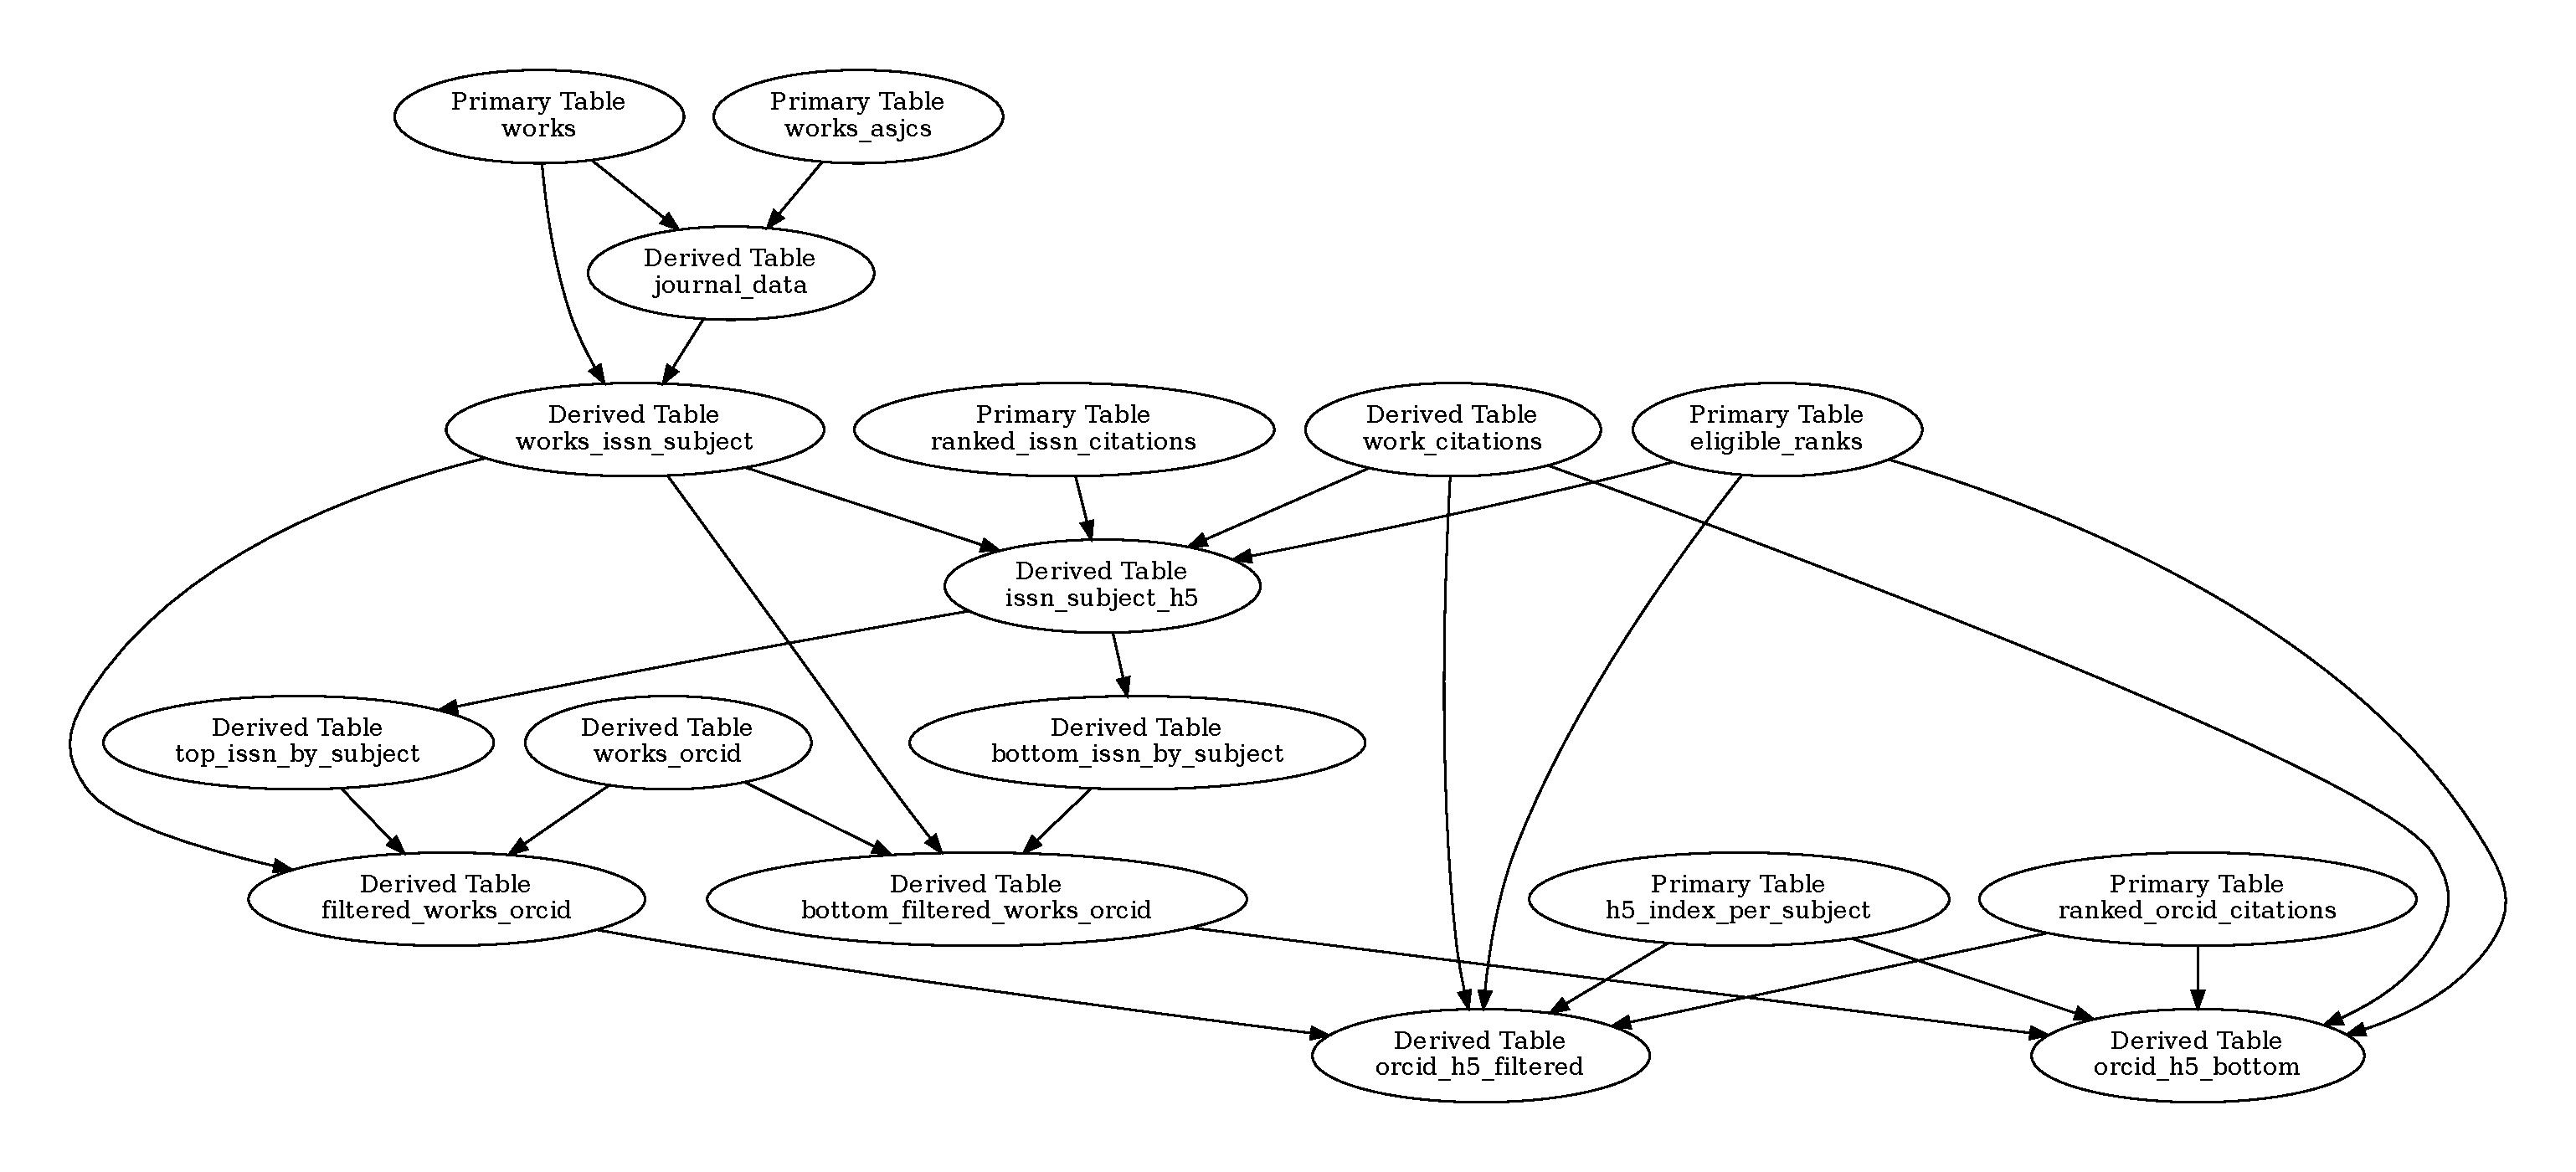
\includegraphics[width=\textwidth]{../figs/full-graph_h5.pdf}
    \caption{Full Dependency graph of the adjusted h5-index calculation with journals filtered using the h5-index}
    \label{fig:dependency_graph_h5}
\end{figure}

\begin{figure}[H]
    \centering
    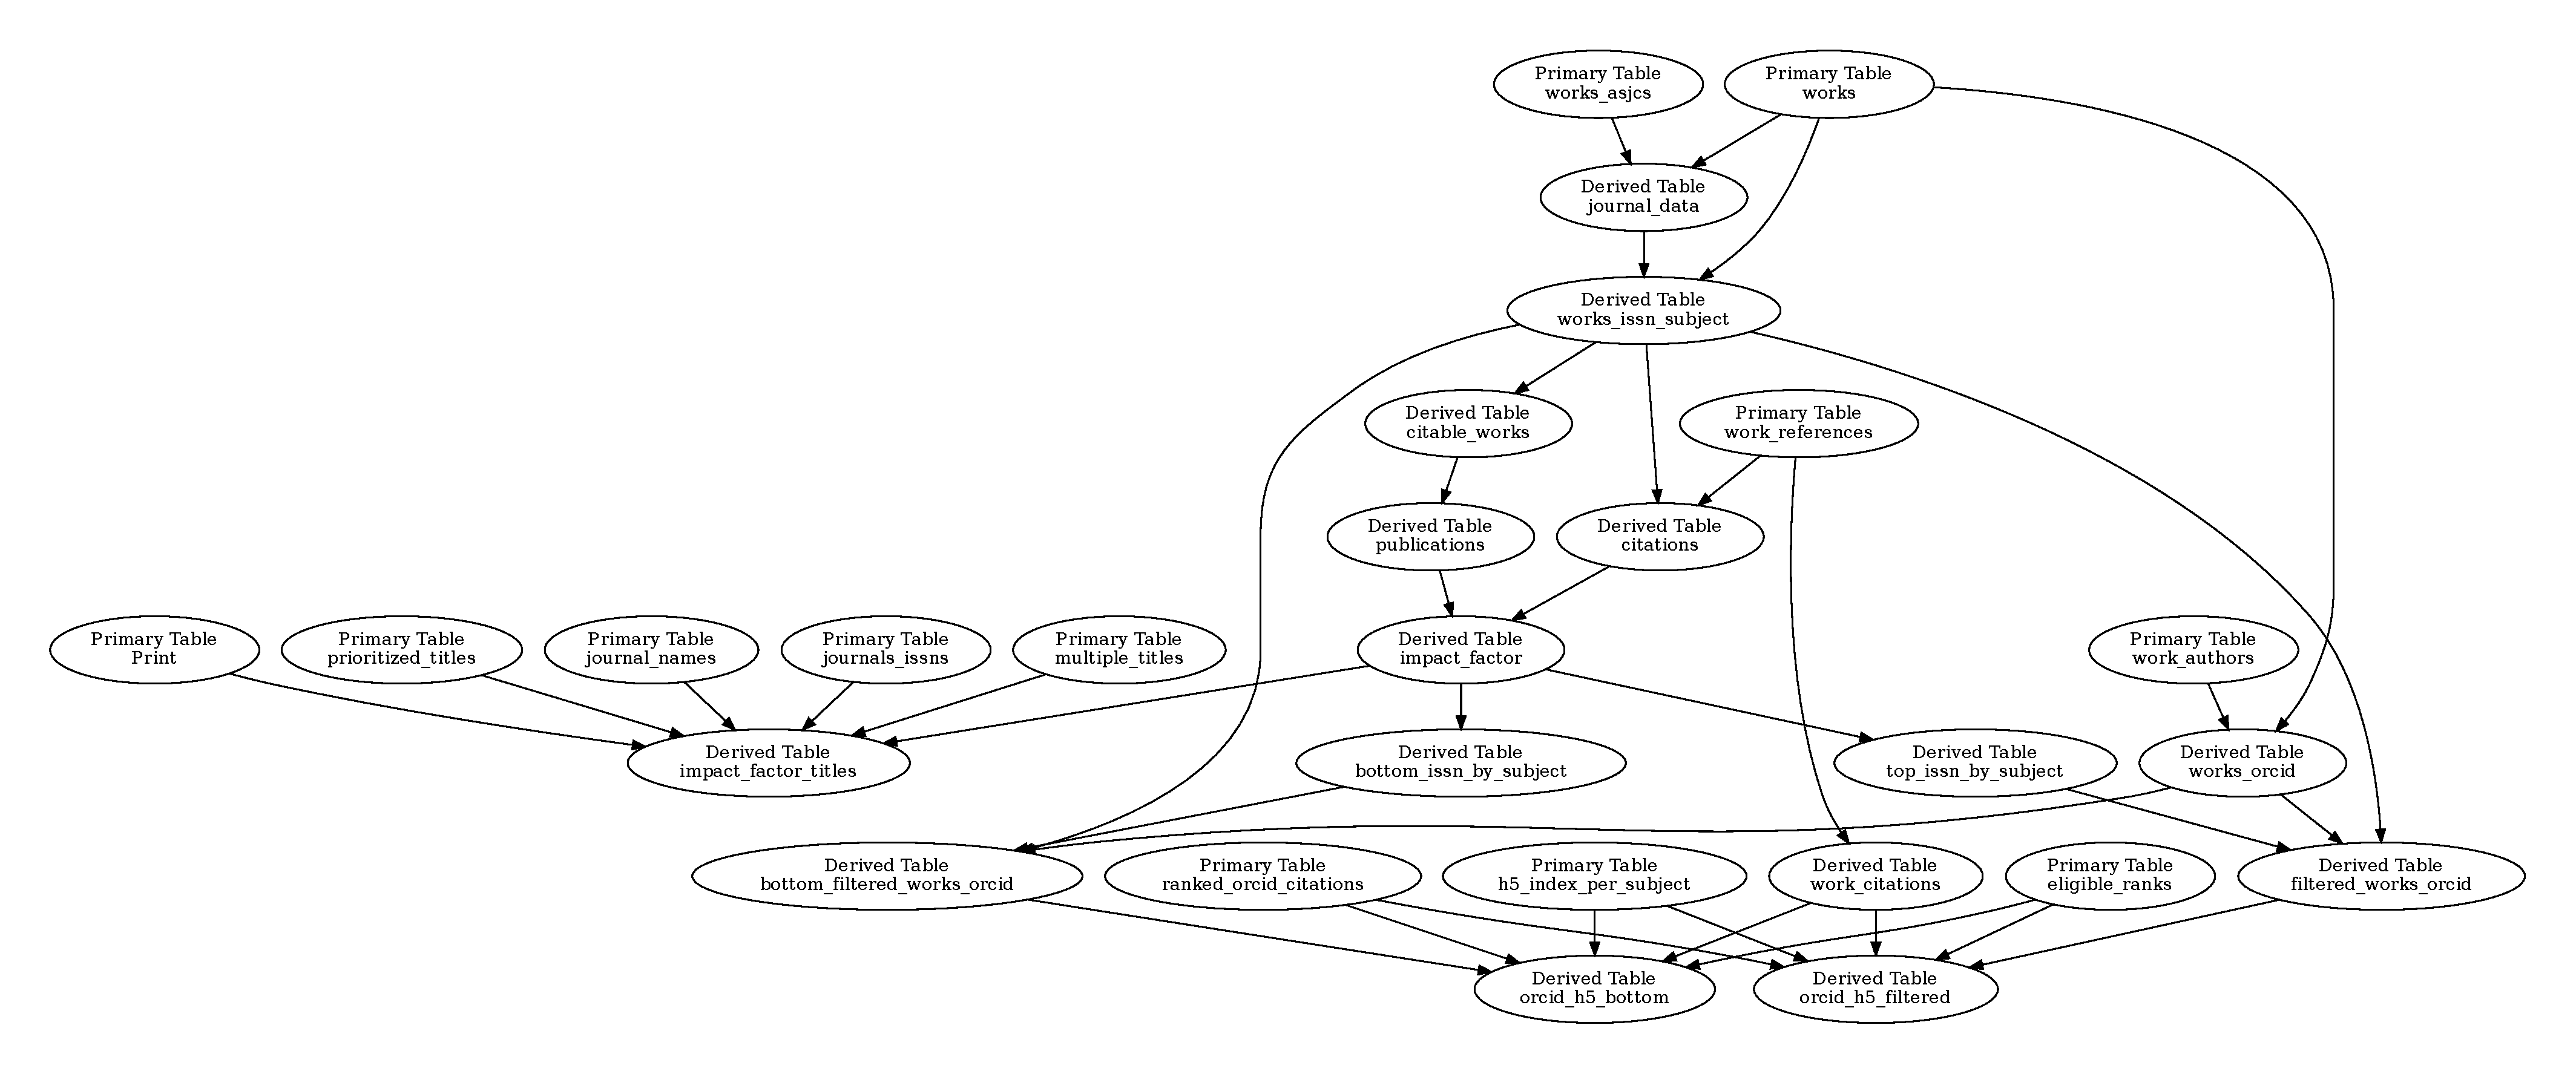
\includegraphics[width=\textwidth]{../figs/full-graph_jif.pdf}
    \caption{Full Dependency graph of the adjusted h5-index calculation with journals filtered using the impact factor}
    \label{fig:dependency_graph_jif}
\end{figure}

\begin{figure}[H]
    \centering
    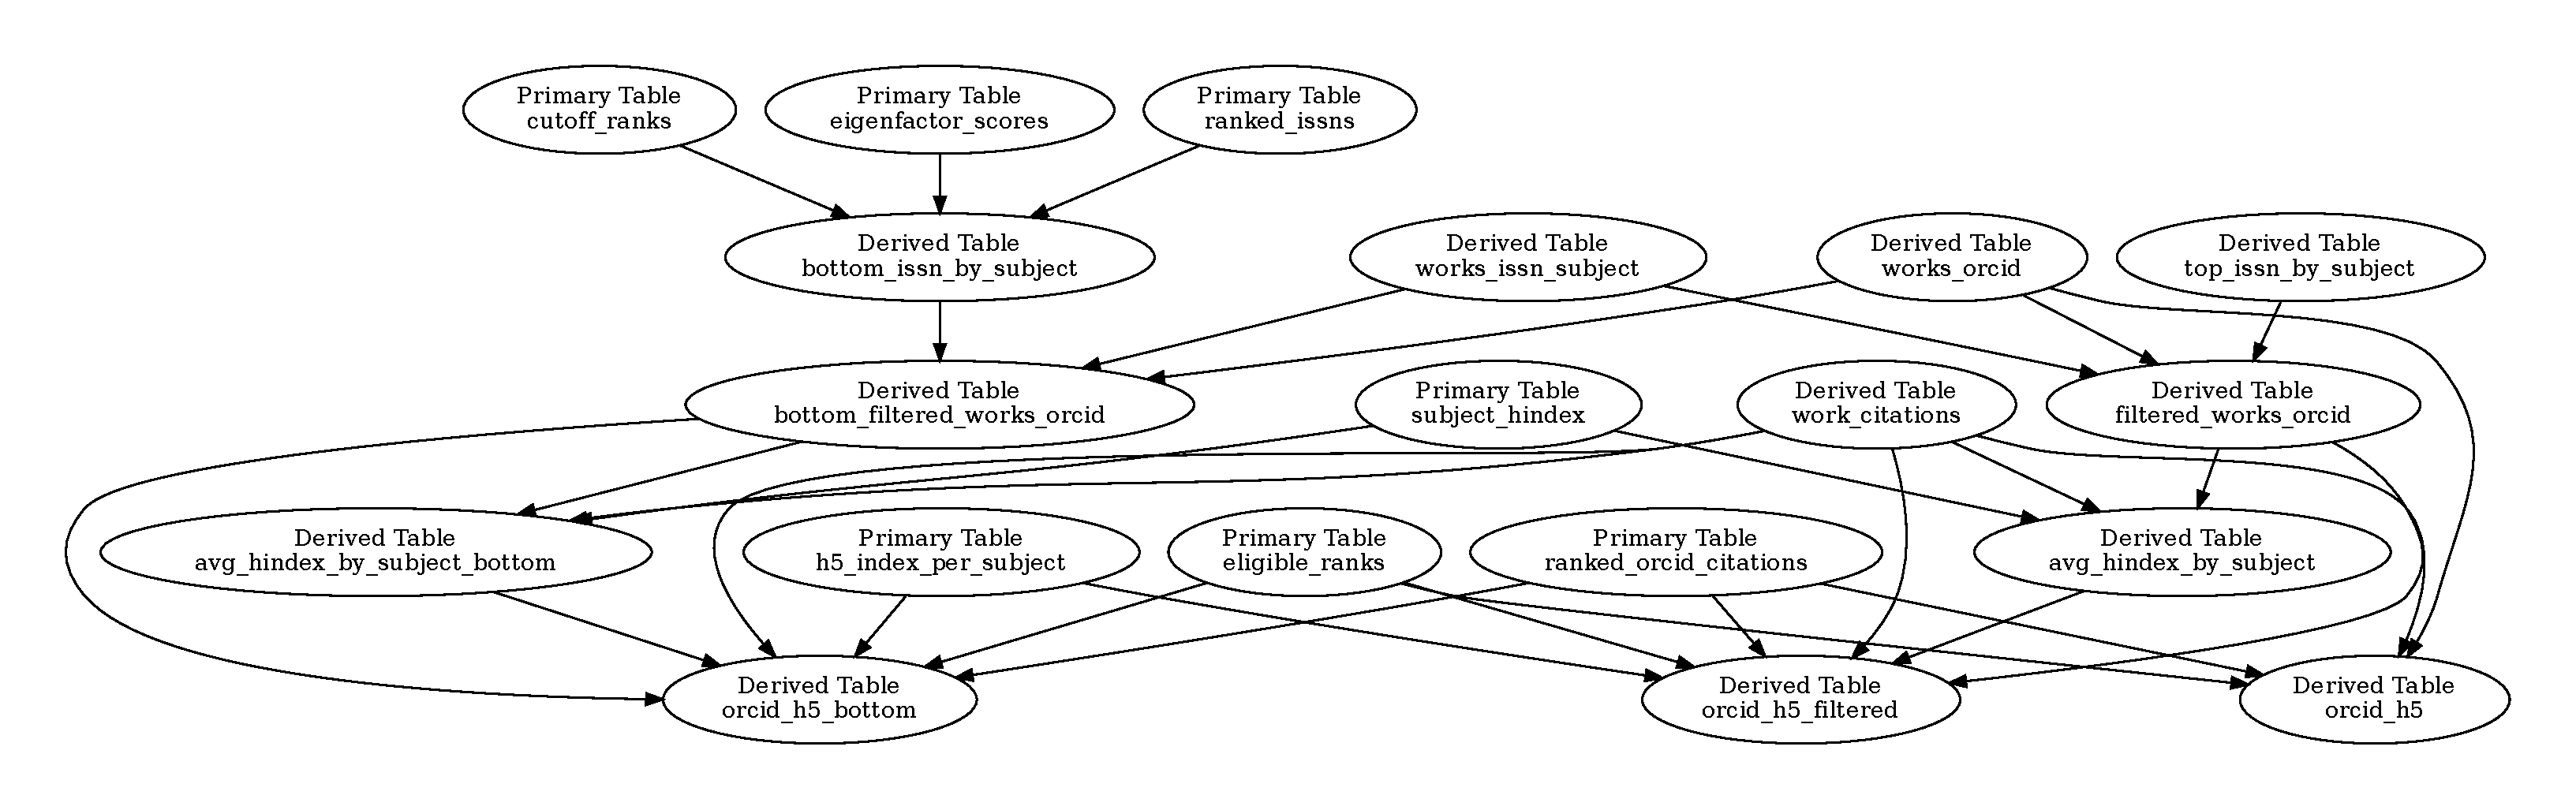
\includegraphics[width=\textwidth]{../figs/full-graph_ef.pdf}
    \caption{Full Dependency graph of the adjusted h5-index calculation with journals filtered using the EigenFactor}
    \label{fig:dependency_graph_ef}
\end{figure}

